\section{La teoría de conjuntos ZFC}

%------------------------------------------------
\subsection{Una nueva teoría de conjuntos}

\begin{frame}
\frametitle{Ernst Zermelo}
\begin{figure}
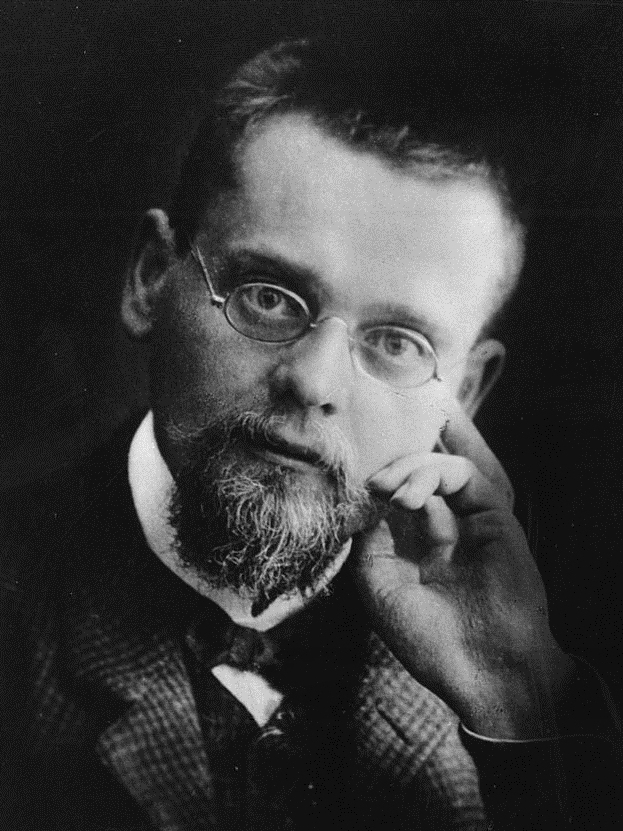
\includegraphics[width=0.5\linewidth]{IMGS/zermelo}
\end{figure}
\end{frame}

%------------------------------------------------

\begin{frame}
\frametitle{Una nueva teoría de conjuntos}

\startchronology
[startyear=1902, stopyear=1928]
%color=black, height=5ex, with=\hsize]
\chronoperiode[startdate=false,stopdate=false,textwidth=3.2cm]{1904}{1908}{\qquad Zermelo;\endgraf 
1904: Buen orden;\endgraf
1908: Axiomas Z} 
%%1er artículo de teoría de conjuntos. Él describe rigurosamente la noción de infinito. Muestra que los infinitos vienen en diferentes tamaños. Prueba el polémico resultado de que casi todos los números son trascendentales.
\chronoperiode[textwidth=2.8cm]{1910}{1919}{\qquad Russell\endgraf
\quad Whitehead}
\chronoevent[textwidth=2.cm]{1922}{~~Axiomas\endgraf
\qquad ZF}
\chronoevent[textwidth=1.5cm]{1926}{\quad Banach-Tarski} 
\stopchronology

\end{frame}


\begin{frame}
 \frametitle{Los axiomas Zermelo-Fraenkel}

\begin{enumerate}
	\item[I]	Extensionalidad: igualdad de conjuntos
	\item[II]	Vacío: existe al menos un conjunto
	\item[III]  Unión: unión de conjuntos
	\item[IV]	Potencia: el conjunto de los subconjuntos
	\item[V]	Infinitud: existe un conjunto infinito
	\item[VI]	Reemplazamiento %fórmulas y evaluaciones
	\item[VII]	Relación de Tipos %implica el ax especificacion
	\item[AC]	Elección%: para cualquier familia de conjuntos el producto cartesiano es no vacío
\end{enumerate}
\end{frame}

\begin{frame}
 \frametitle{Resolviendo la paradoja de Rusell}

\textbf{Axioma del Esquema de Comprensión (FALSO)}. Si $P$ es una propiedad, entonces existe un conjunto $Y = \{x: P(x)\}$.\\~

\pause
Y el conjunto de todos los conjuntos no existe, en todo caso: 
\begin{center}
 ¡¡ es el concepto del conjunto de todos los conjuntos lo que es paradójico, no la idea misma de la comprensión de un conjunto !!
\end{center}
\end{frame}

\begin{frame}
 \frametitle{El Buen Orden}
 
\justify
Todo subconjunto de los números naturales se puede ordenar en el sentido intuitivo.\\

\pause
El concepto del buen orden generaliza la propiedad de buen orden de los naturales y da origen a la teoría de los números ordinales.
 
\pause
\begin{block}{Principio del Buen Orden}
  Todo subconjunto, no vacío, de naturales admite un primer elemento.
\end{block}
\end{frame}

\begin{frame}
 \frametitle{El Buen Orden}

\justify
La noción de orden abstracta se define apelando a la noción de subcojunto.\\

\pause
 \begin{theorem}[Teorema del Buen Orden]
  Todo subconjunto no vacío de naturales admite un primer elemento.
 \end{theorem}
 
 \pause
 \begin{proof}
  \begin{center}
  ¡¡Requiere hacer uso de un axioma adicional, el Axioma de Elección!!
  \end{center}
 \end{proof}
\end{frame}

\subsection{El Axioma de Elección}

\begin{frame}
 \frametitle{El Axioma de Elección}
 
 \begin{figure}
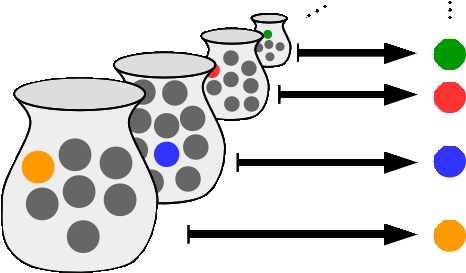
\includegraphics[width=0.7\linewidth]{IMGS/choice}
\end{figure}
\end{frame}
  
 \begin{frame}
 \frametitle{La paradoja de Banach-Tarski}
 
 \begin{theorem}
  Es posible dividir una esfera de radio $1$ en ocho partes disjuntas dos a dos, de modo que, aplicando movimientos oportunos a cinco de ellas, obtengamos 
  nuevos conjuntos que constituyan una partición de una esfera de radio $1$, y lo mismo ocurra con las tres partes restantes.
 \end{theorem}
\end{frame}

\begin{frame}
 \frametitle{La paradoja de Banach-Tarski}
 
 \begin{figure}
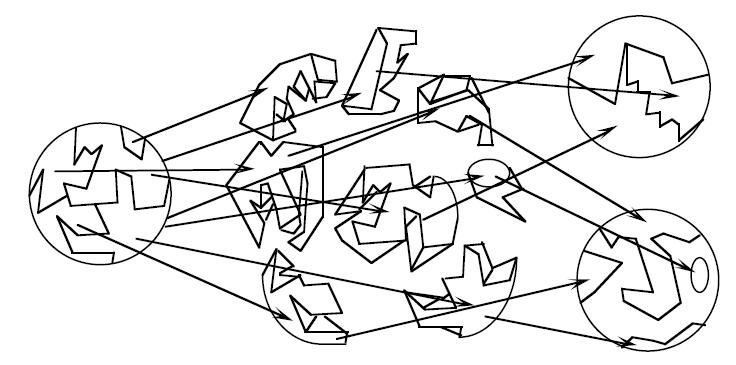
\includegraphics[width=1.\linewidth]{IMGS/tarski}
\end{figure}
\end{frame}

%------------------------------------------------
\subsection{Consistencia y completitud de la teoría ZFC}

\begin{frame}
\frametitle{Godel y Cohen}

\begin{columns}[c]

\column{.5\textwidth} 
\begin{figure}
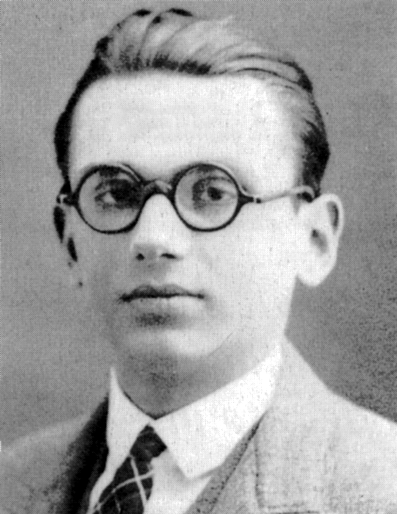
\includegraphics[width=0.7\linewidth]{IMGS/godel}
\end{figure}

\column{.5\textwidth} 
\begin{figure}
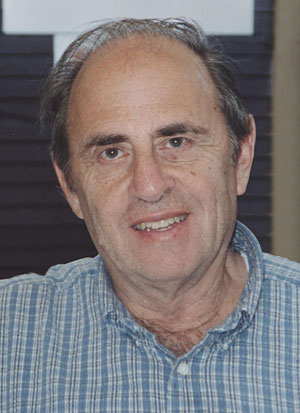
\includegraphics[width=0.7\linewidth]{IMGS/cohen}
\end{figure}

\end{columns}
\end{frame}

%------------------------------------------------

\begin{frame}
\frametitle{Goedel y Cohen}

\startchronology
[startyear=1930, stopyear=1965]
\chronoevent[textwidth=1.8cm]{1931}{ ~~Goedel\endgraf
Incompletitud} 
\chronoperiode[startdate=false]{1934}{1935}{~~Zorn}
\chronoevent[textwidth=1.5cm]{1940}{\quad Goedel\endgraf
Consistencia}
\chronoevent[textwidth=1.5cm]{1963}{\quad Cohen}
\stopchronology

\end{frame}

%------------------------------------------------

\begin{frame}
 \frametitle{Equivalencias al Axioma de Elección}
 
 \begin{itemize}
  \item Principio Multiplicativo
  \item Principio de Buen Orden
  \item El Lema de Zorn
  \item Principio de Kuratowski
 \end{itemize}
\end{frame}

\begin{frame}
 \frametitle{Aplicaciones del Axioma de Elección}
 
 \begin{itemize}
  \item Todo espacio vectorial tiene una base (Álgebra Lineal).
  \item La unión enumerable de conjuntos enumerables es enumerable.
  \item Existe un conjunto de números reales que no es Lebesgue-medible (Teoría de la Medida).
  \item El producto de espacios compactos es compacto (Topología).
  \item Todo anillo con unidad tiene un ideal maximal (Álgebra).
  \item Todo orden parcial puede extenderse a un orden total.
  \item El teorema de Hahn-Banach (Análisis Funcional).
  \item El teorema de completud para la lógica de primer orden.
  \item Toda álgebra de Boole es isomorfa a un campo de conjuntos.
 \end{itemize}
\end{frame}

\begin{frame}
 \frametitle{El axioma de elección (AC) y ZF}
 
 \begin{theorem}
  Bajo la teoría ZF, el axioma de elección es equivalente a la hipótesis del continuo generalizado.
 \end{theorem}
 
 \pause
 \begin{theorem}[Indecibilidad; \cite{godel1938consistency}]
  El axioma de elección y la hipótesis del continuo generalizado es consistente de los axiomas de la teoría de conjuntos ZF.
 \end{theorem}
 %no puede refutarse con ZF
 
 \pause
 \begin{theorem}[Independencia; \cite{cohen2008set}]
  El axioma de elección y la hipótesis del continuo generalizado es independiente de los axiomas de la teoría de conjuntos ZF.
 \end{theorem}
 %no puede probarse con ZF
\end{frame}


\begin{frame}
\frametitle{Una teoría de conjuntos estándar}

\begin{alertblock}{Teoría ZFC}
	\justify
	La teoría de conjuntos es uno de los mayores logros de la matemática moderna. Básicamente todos los conceptos matemáticos, métodos y resultados admiten la representación dentro de la teoría axiomática de conjuntos.
\end{alertblock}

%Forzamos citaciones fantasmas
\nocite{jech2003set,kuratowski2014introduction,pickover2009math,herrlich2006axiom}.
\end{frame}